
\begin{wrapfigure}{R}{0.5\linewidth}
\vskip -0.18in
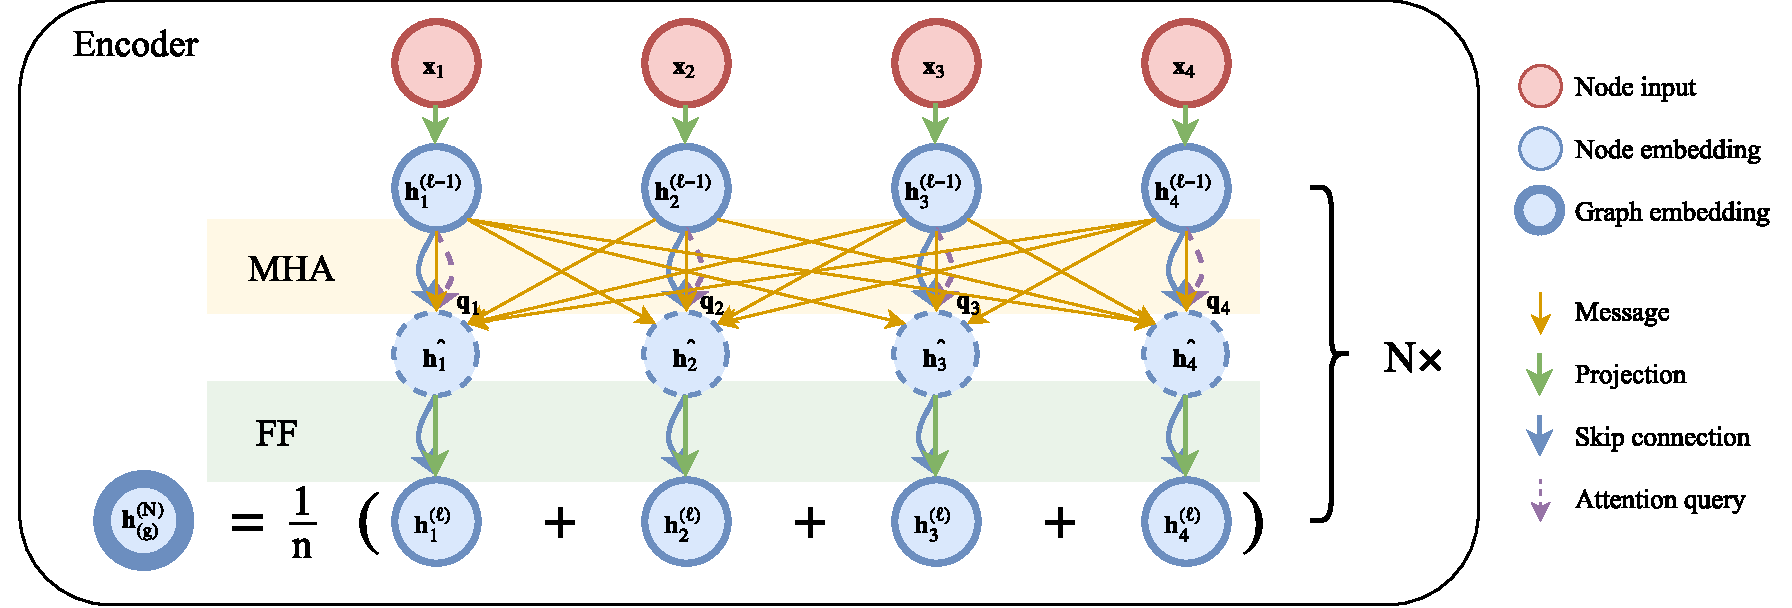
\includegraphics[trim={0 1.0 0 0.0},clip,width=1.0\linewidth]{./images/Encoder}
\vskip -0.06in
\caption{Attention based encoder. Input nodes are embedded and processed by $N$ sequential layers, each consisting of a multi-head attention (MHA) and node-wise feed-forward (FF) sublayer. The graph embedding is computed as the mean of node embeddings. Best viewed in color.}
\label{fig:encoder}
\vskip -0.1in
\end{wrapfigure}

\section{Attention model}
\label{sec:attention_model}
We define the Attention Model in terms of the TSP. For other problems, the model is the same but the input, mask and decoder context need to be defined accordingly, which is discussed in the Appendix.
We define a problem instance $s$ as a graph with $n$ nodes, where node $i \in \{1, \ldots, n\}$ is represented by features $\mathbf{x}_i$. For TSP, $\mathbf{x}_i$ is the coordinate of node $i$ and the graph is fully connected (with self-connections) but in general, the model can be considered a Graph Attention Network \citep{velickovic2018graph} and take graph structure into account by a masking procedure (see Appendix \ref{sec:appendix_attention_model_details}). We define a solution (tour) $\bm{\pi} = (\pi_1, \ldots, \pi_n)$ as a permutation of the nodes, so $\pi_t \in \{1, \ldots n\}$ and $\pi_t \neq \pi_{t'} \, \forall t \neq t'$.
Our attention based encoder-decoder model defines a stochastic policy $p(\bm{\pi}|s)$ for selecting a solution $\bm{\pi}$ given a problem instance $s$. It is factorized and parameterized by $\bm{\theta}$ as
\begin{equation}
\label{eq:p_model}
	p_\theta(\bm{\pi}|s) = \prod\limits_{t=1}^{n} p_{\bm{\theta}}(\pi_t|s, \bm{\pi}_{1:t-1}).
\end{equation}
The encoder produces embeddings of all input nodes. The decoder produces the sequence $\bm{\pi}$ of input nodes, one node at a time. It takes as input the encoder embeddings and a problem specific mask and context. For TSP, when a partial tour has been constructed, it cannot be changed and the ‘remaining’ problem is to find a path from the last node, through all unvisited nodes, to the first node. The order and coordinates of other nodes already visited are irrelevant. To know the first and last node, the decoder context consists (next to the graph embedding) of embeddings of the first and last node. Similar to \citet{bello2016neural}, the decoder observes a mask to know which nodes have been visited.



\subsection{Encoder}
The encoder that we use (Figure \ref{fig:encoder}) is similar to the encoder used in the Transformer architecture by \citet{vaswani2017attention}, but we do not use positional encoding such that the resulting node embeddings are invariant to the input order. From the $d_{\text{x}}$-dimensional input features $\mathbf{x}_i$ (for TSP $d_{\text{x}}$ = 2), the encoder computes initial $d_{\text{h}}$-dimensional node embeddings $\mathbf{h}_i^{(0)}$ (we use $d_{\text{h}} = 128$) through a learned linear projection with parameters $W^{\text{x}}$ and $\mathbf{b}^{\text{x}}$: $\mathbf{h}_i^{(0)} = W^{\text{x}} \mathbf{x}_i + \mathbf{b}^{\text{x}}$.
The embeddings are updated using $N$ attention layers, each consisting of two sublayers. We denote with $\mathbf{h}_i^{(\ell)}$ the node embeddings produced by layer $\ell \in \{1, .., N\}$. The encoder computes an aggregated embedding $\bar{\mathbf{h}}^{(N)}$ of the input graph  as the mean of the final node embeddings $\mathbf{h}_i^{(N)}$: $\bar{\mathbf{h}}^{(N)} = \frac{1}{n} \sum_{i = 1}^n \mathbf{h}_i^{(N)}$.
Both the node embeddings $\mathbf{h}_i^{(N)}$ and the graph embedding $\bar{\mathbf{h}}^{(N)}$ are used as input to the decoder.

\paragraph{Attention layer}
Following the Transformer architecture \citep{vaswani2017attention}, each attention layer consist of two sublayers: a multi-head attention (MHA) layer that executes message passing between the nodes and a node-wise fully connected feed-forward (FF) layer. Each sublayer adds a skip-connection \citep{he2016deep} and batch normalization (BN) \citep{ioffe2015batch} (which we found to work better than layer normalization \citep{ba2016layer}): 
\begin{align}
	 \hat{\mathbf{h}}_i & =\text{BN}^{\ell}\left( \mathbf{h}_i^{(\ell-1)} + \text{MHA}_i^{\ell}\left( \mathbf{h}_1^{(\ell-1)}, \ldots, \mathbf{h}_n^{(\ell-1)}\right)\right) \label{eq:attn_sublayer1} \\
    \mathbf{h}_i^{(\ell)} & =\text{BN}^{\ell}\left(\hat{\mathbf{h}}_i + \text{FF}^{\ell}(\hat{\mathbf{h}}_i)\right). \label{eq:attn_sublayer2}
\end{align}
The layer index $\ell$ indicates that the layers do \emph{not} share parameters. The MHA sublayer uses $M = 8$ heads with dimensionality $\frac{d_h}{M}=16$, and the FF sublayer has one hidden (sub)sublayer with dimension 512 and ReLu activation. See Appendix \ref{sec:appendix_attention_model_details} for details.

\begin{figure*}[t]
\begin{center}
\centerline{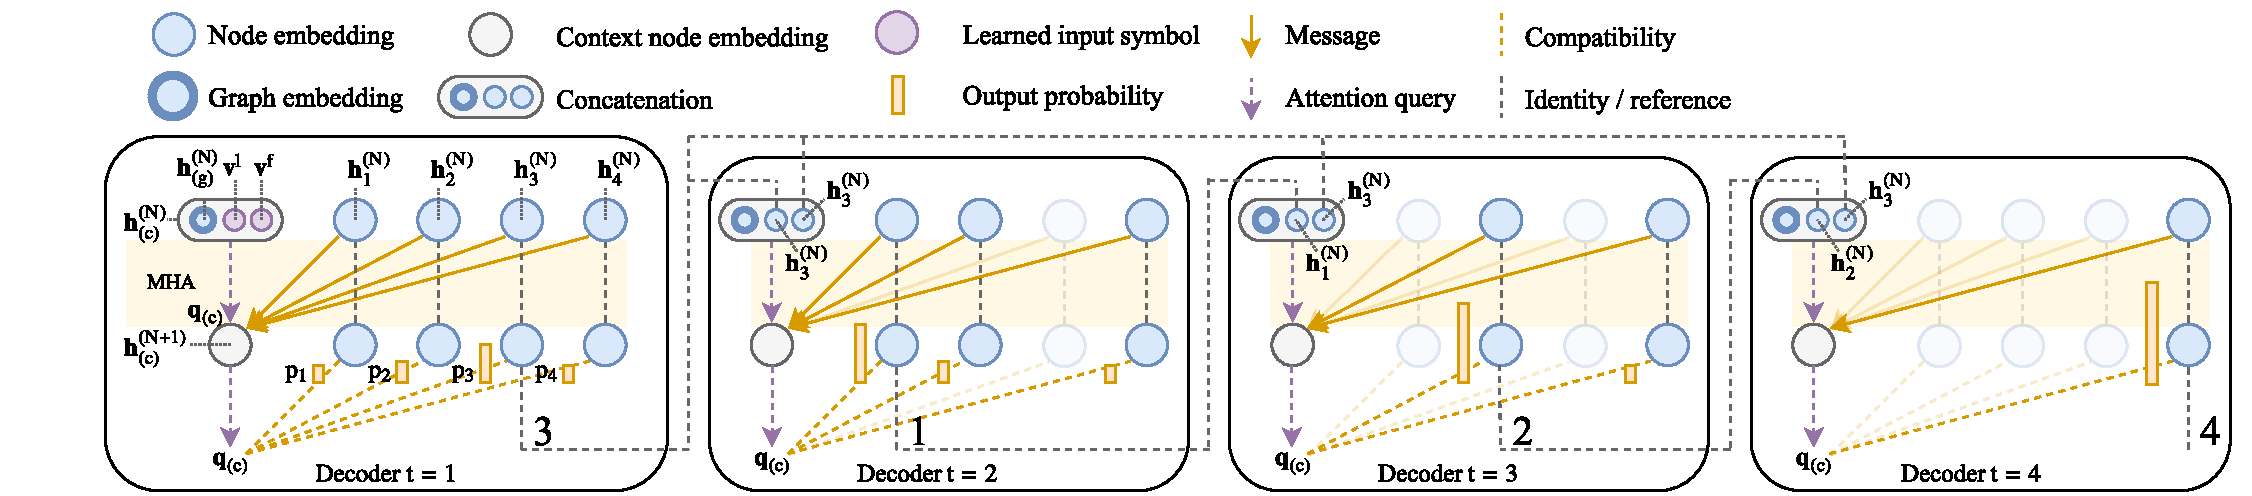
\includegraphics[trim={50 0 0 0},clip,width=\textwidth]{./images/Decoder}}
\caption{Attention based decoder for the TSP problem. The decoder takes as input the graph embedding and node embeddings. At each time step $t$, the context consist of the graph embedding and the embeddings of the first and last (previously output) node of the partial tour, where learned placeholders are used if $t = 1$. Nodes that cannot be visited (since they are already visited) are masked. The example shows how a tour $\bm{\pi} = (3, 1, 2, 4)$ is constructed. Best viewed in color.}
\label{fig:decoder}
\end{center}
\vskip -0.2in
\end{figure*}

\subsection{Decoder}
Decoding happens sequentially, and at timestep $t \in \{1, \ldots n\}$, the decoder outputs the node $\pi_t$ based on the embeddings from the encoder and the outputs $\pi_{t'}$ generated at time $t' < t$. During decoding, we augment the graph with a special \emph{context node} $(c)$ to represent the decoding context. The decoder computes an attention (sub)layer on top of the encoder, but with messages only to the context node for efficiency.\footnote{$n \times n$ attention between all nodes is expensive to compute in every step of the decoding process.} The final probabilities are computed using a single-head attention mechanism. See Figure \ref{fig:decoder} for an illustration of the decoding process.

\paragraph{Context embedding}
The context of the decoder at time $t$ comes from the encoder and the output up to time $t$. As mentioned, for the TSP it consists of the embedding of the graph, the previous (last) node $\pi_{t-1}$ and the first node $\pi_1$. For $t = 1$ we use learned $d_{\text{h}}$-dimensional parameters $\mathbf{v}^\text{l}$ and $\mathbf{v}^\text{f}$ as input placeholders:
\begin{equation}
	\mathbf{h}_{(c)}^{(N)} = \begin{cases}
		\left[\bar{\mathbf{h}}^{(N)} , \mathbf{h}^{(N)}_{\pi_{t-1}} , \mathbf{h}^{(N)}_{\pi_1}\right] & t > 1 \\
        \left[\bar{\mathbf{h}}^{(N)} , \mathbf{v}^\text{l} , \mathbf{v}^\text{f}\right] & t = 1.
\end{cases} \\
\end{equation}
Here $[\cdot,\cdot,\cdot]$ is the horizontal concatenation operator and we write the $(3 \cdot d_{\text{h}})$-dimensional result vector as $\mathbf{h}_{(c)}^{(N)}$ to indicate we interpret it as the embedding of the special context node $(c)$ and use the superscript $(N)$ to align with the node embeddings $\mathbf{h}_i^{(N)}$. We could project the embedding back to $d_{\text{h}}$ dimensions, but we absorb this transformation in the parameter $W^Q$ in \eqref{eq:dec_qkv}.

Now we compute a new context node embedding $\mathbf{h}_{(c)}^{(N+1)}$ using the ($M$-head) attention mechanism described in Appendix \ref{sec:attention_mechanism}. The keys and values come from the node embeddings $\mathbf{h}_i^{(N)}$, but we only compute a single query $\mathbf{q}_{(c)}$ (per head) from the context node (we omit the $(N)$ for readability):
\begin{equation}
\label{eq:dec_qkv}
	\mathbf{q}_{(c)} = W^Q \mathbf{h}_{(c)} \quad \mathbf{k}_i = W^K \mathbf{h}_i, \quad \mathbf{v}_i = W^V \mathbf{h}_i.
\end{equation}
We compute the compatibility of the query with all nodes, and mask (set $u_{(c)j} = -\infty$) nodes which cannot be visited at time $t$. For TSP, this simply means we mask the nodes already visited:
\begin{equation}
\label{eq:dec_compatibility}
	u_{(c)j} = \begin{cases}
		\frac{\mathbf{q}_{(c)}^T \mathbf{k}_j}{\sqrt{d_{\text{k}}}} & \text{if } j \neq \pi_{t'} \quad \forall t' < t \\
        -\infty & \text{otherwise.}
    \end{cases}
\end{equation}
Here $d_{\text{k}} = \frac{d_{\text{h}}}{M}$ is the query/key dimensionality (see Appendix \ref{sec:appendix_attention_model_details}). Again, we compute $u_{(c)j}$ and $\mathbf{v}_i$ for $M = 8$ heads and compute the final multi-head attention value for the context node using equations \plaineqref{eq:attention_weights}--\plaineqref{eq:MHA} from Appendix \ref{sec:appendix_attention_model_details}, but with $(c)$ instead of $i$. This mechanism is similar to our encoder, but does not use skip-connections, batch normalization or the feed-forward sublayer for maximal efficiency. The result $\mathbf{h}_{(c)}^{(N+1)}$ is similar to the \emph{glimpse} described by \citet{bello2016neural}.

\paragraph{Calculation of log-probabilities}
To compute output probabilities $p_{\bm{\theta}}(\pi_t|s, \bm{\pi}_{1:t-1})$ in \eqref{eq:p_model}, we add one final decoder layer with a \emph{single} attention head ($M=1$ so $d_{\text{k}} = d_{\text{h}}$). For this layer, we \emph{only} compute the compatibilities $u_{(c)j}$ using \eqref{eq:dec_compatibility}, but following \citet{bello2016neural} we clip the result (before masking!) within $[-C, C]$ (C = 10) using $\tanh$:
\begin{equation}
\label{eq:dec_logits}
	u_{(c)j} = \begin{cases}
		C \cdot \tanh \left(\frac{\mathbf{q}_{(c)}^T \mathbf{k}_j}{\sqrt{d_{\text{k}}}}\right) & \text{if } j \neq \pi_{t'} \quad \forall t' < t \\
        -\infty & \text{otherwise.}
    \end{cases}
\end{equation}
We interpret these compatibilities as unnormalized log-probabilities (logits) and compute the final output probability vector $\mathbf{p}$ using a softmax (similar to \eqref{eq:attention_weights} in Appendix \ref{sec:appendix_attention_model_details}):
\begin{equation}
	\label{dec:probabilities}
    p_i = p_{\bm{\theta}}(\pi_t = i|s, \bm{\pi}_{1:t-1}) = \frac{e^{u_{(c)i}}}{\sum_{j}{e^{u_{(c)j}}}}.
\end{equation}